\section*{Discussion}
\wt{Honestly, I do not really think you need this last part (future work) given space limitation (watch out the total number of words and references). Instead I would rather develop some of the already written part that remains a bit vague and imprecise to me. I added few things to see what I mean. }
\aa{Discussion: the section ‘Advantages of model integration’, which I wrote, and ‘Applicability of the method’ have several points in common. Maybe they could be merged into a single section: ‘Applicability and advantages of model integration’. Maybe, it should be discussed more extensively how to face the situation in which predictions of correlative model and sub-models are so different that the integrated model performs poorer than the two (I mean, does that mean that the approach is not valid in those cases?)
I liked a lot the idea of adding Figure 6. The link between this approach and adaptive management seems to me one of its biggest advantages. The box in the right could maybe just say: 'monitoring of management actions’? }

\subsection*{Comparison with other methods}
\ab{The methods provided here expand upon the motivation of hybrid models to develop a more robust and unifying approach for ecological models in a predictive context while striving to overcome some of the limitations characteristic of other integrated approaches. 
Attempting to incorporate the underlying ecological processes so that SDMs are not oversimplified by combining different model parameters or scales can pose a challenge to these hybrid approaches. 
In particular, it can often be difficult to identify parameters that can be used to connect different modelling frameworks and what parameters can produce purposeful responses \citep{Thuiller2013}. 
The methods presented in this study aim to overcome some of these limitations through the use of Bayesian statistics. 
Bayesian methods allow for the inclusion of prior information and produce results as an entire distribution instead of a single point aiding in the reduction of error propagation \citep{Kery2010}. 
The estimation of a response as an entire distribution helps to decrease over parameterization that is a concern for hybrid models and thereby also provides a more comprehensible response for reporting results. 
Bayesian frameworks provide a natural framework for the incorporation of prior information. 
The inability or difficulty to include information from experimental studies or ecological processes at lower scales can be a possible drawback of hybrid models \citep{Thuiller2008, Smolik2010}. 
Even when a link can be formed to include this information, it often is oversimplified to simplify computing \citep{Gallien2010}. 
Bayesian methods therefore provide a reasonable alternative to allow for the easy unification of previous experimental studies or other prior information. Finally, Bayesian methods inherently allow for feedbacks or interactions between sub models, which may portray a more realistic response to many environmental dynamics where factors may simultaneously influence the change of one another.}
\mt{Maybe change Kery citation to Link \& Barker}

Our approach is an original application of Bayesian multilevel modelling, and can be considered a logical extension of other Bayesian approaches developed to deal with processes that occur at multiple scales while using several models simultaneously. 
In particular, this development has certain similarities with Bayesian model averaging, Bayesian calibration of process-based models and hierarchical Bayesian modelling. 
Bayesian model averaging aims to combine several alternative models to obtain better predictions while taking into account parameter uncertainties \citep{Hoeting1999}, and has been applied numerous times in ecology where the mechanisms underlying a complex phenomenon are often unknown \citep[e.g.][]{Wintle2003, Link2006}. 
Bayesian model averaging considers models operating at the same scale and the posterior distribution is usually determined with Gibbs sampling. 
Bayesian calibration of process-based model focuses on uncertainty of the parameter values in the process-based models, in this case the values of the parameters are calibrated by the model output \citep{VanOijen2005, VanOijen2011}. 
\wt{Hartig, F., Dyke, J., Hickler, T., Higgins, S.I., O'Hara, R.B., Scheiter, S. \& Huth, A. (2012) Connecting dynamic vegetation models to data - an inverse perspective. Journal of Biogeography, 39, 2240-2252.}
In contrast with Bayesian model averaging and calibration techniques, our approach handles data and models operating at different hierarchical scales, and uses process-based models to constrain the shape of a generally more correlative meta-model.
Similar hierarchical approaches have been applied to diverse fields, including engineering \citep{Booth2013}, hydraulic conductivity models \citep{Dostert2009, Efendiev2005, Efendiev2005a}, plant physiology \citep{Ogle2008, Ogle2009}, and climate and atmospheric modelling \citep{Zimmerman2005, Mcmillan2010, Kang2012}.
\wt{Why not being more precise and exploratory here. You may actually run a model averaging around your approach, may not you? Indeed, if we think to Ex 1 you could have several native meta-model posterior distributions, right? Or even a direct model averaging from them. As said, you could actually run something like biomod2 to get the distribution of values for each pixel given the models/algorithms and data and use them directly as a posterior into the integration. . 
The integration could also be done in the Ex 2 as far as I could see it. 
It might nicely link your approach to the on-going move of SDM people towards ensemble modeling and forecasting. It also lonk to Bayesian model averaging. 
If I was meant, I would say that a simple use of binomial GLM is a 10-years way back for most people where more 
}

\subsection*{Advantages of Model Integration}
Models are important tools that are increasingly used by land managers to face challenges associated to decision-making. 
A growing number of models are available, but they can provide diverging answers to very similar questions due to the differences in their assumptions and methodology. 
This can create confusion and even some mistrust towards models, and as a consequence some managers may be discouraged to incorporate any model at all in their management plans. 
By integrating different types of models---and their outputs---into a common framework, we believe that our approach can contribute to overcome the gap between modelers and practitioners and thus promote more widespread use of models to support decision-making.
\ia{This is repetitive with the applicability section. I suggest that you stick here on the modeling advantage of your approach and keep the applied advantage for the other section}

\ia{suggest adding here:\\
Model uncertainties is another key factor affecting applicability of model outputs (Addison et al., 2013). }
Our approach also allows for a clear, transparent identification of uncertainties and how they are transmitted throughout the modelling process. 
\tf{Really? I thought that only the uncertainty in the predictions are available and not the uncertainty from submodels.}
This is one of the main strengths of this approach, and offers several advantages. 
For instance, transparency in uncertainty can be considered as a sort of sensitivity analysis, in which areas with large uncertainty can be detected and new experimental research or additional data collection can be designed (e.g., Example 1, Figs. \ref{fig:ex1_sampling}, \ref{fig:ex1_precip}).
The new knowledge resulting from this research can be readily incorporated into the metamodel, allowing for an iterative learning process that will undoubtedly contribute to reduce uncertainty in predictions for a wide range of environmental conditions. 
\tf{The question is also: which model do we aim to incorporate. At a point, incorporating a model maybe useless. }
Moreover, our framework embraces change as a fundamental process and is able to adapt and respond to it. 
The ease of incorporating new knowledge to the modelling framework (including new theory or the result of management and experimental efforts), will allow for a rapid adjustment of the predictions and the incorporation of the most recent available knowledge into management plans. 
In an era of continuous and unprecedented change, adaptive approaches such as the one presented here are often highlighted as a pressing need in order to develop strategies to promote ecosystems that are both feasible and resilient \citep[Fig. \ref{fig:adaptive_management};][]{Seastedt2008, Mori2013}.
\wt{
Perhaps we could also be more precise here. Give examples. Since you are working with forest data, an easy step forward would also be to calibrate growth curve of most tree species in function of both temp and precipitation, even a competition model (see Kunstler et al. 2011 J. of Ecology), that can then be integrated into SDMs. 
Similarly you may also discuss about the NEON and LTER long term sites that could certainly give similar information than the one used in Ex 1. I think we should strenghen the different possibilities to make sure users find the approach useful. It remains to vague to me at this point. 
If you think about the Cheaib et al. paper, you may also suggest that your approach could be run over all different model outputs to integrate thema all together. 
In a way that should re-inforce the link between modellers and long term experimental ecologists that did not really discuss so far since it was difficult to integrate the two informations. 
}
%==================
% FIGURE

\begin{figure}[tb]
	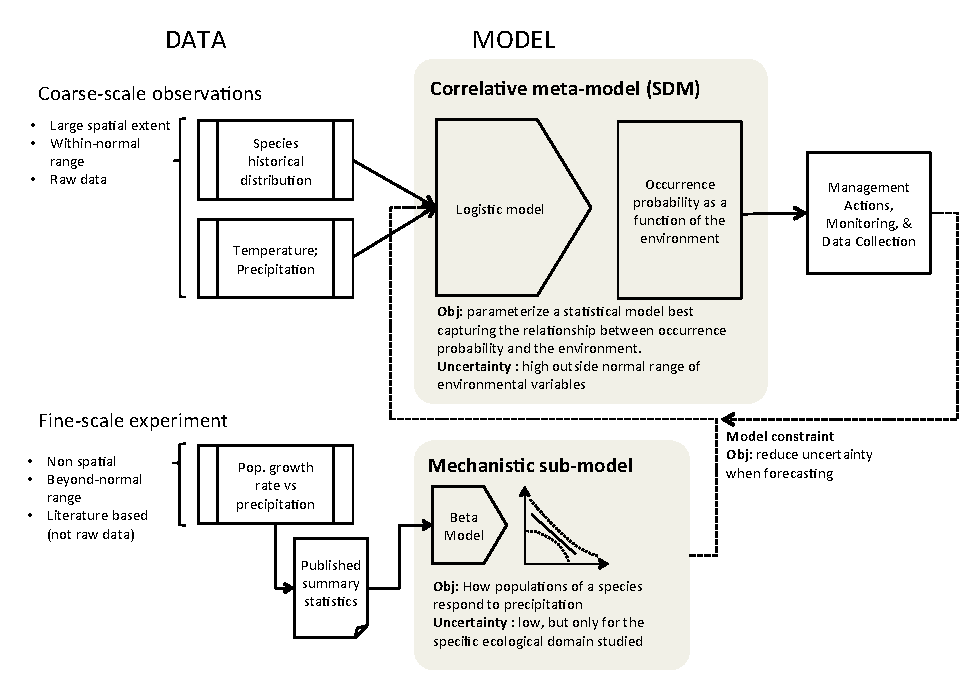
\includegraphics{adaptive_management.pdf}
	\caption{Sample workflow for applying the models presented in the first example in an adaptive management context.
	Critical steps include specifying the meta-model, identifying additional sources of information to be used as constraints on the meta-model, and using the integrated prediction for decision-making.
	As additional information becomes available from monitoring the results of management, this information can be incorporated in additional sub-models to further refine the meta-model.}
	\label{fig:adaptive_management}
\end{figure}

% ERUGIF
%==================


\subsection*{Challenges} 
Although our approach is highly flexible and can be applied in a number of situations, there are some challenges to successfully using the framework.
As with any modelling effort, good model specification with strong links to theory are essential \citep{Austin2007}.
Poorly specified models will produce outputs that are uninformative or misleading, and model integration is not a cure for these problems.
In the worst case, constraining a meta-model with a poor sub-model can result in outcomes that are worse in terms of bias and uncertainty than those produced by a naive model.
We expect model selection will play an important role in applications of our framework, and such schemes can be incorporated relatively easily \citep{Madigan1995, Wasserman2000, Tenan2014}.

In a similar fashion, the quality and availability of data imposes a significant constraint on the number and type of models that can be implemented.
The capacity to implement a model is very low if data requirements are prohibitive. 
Adequate coverage of explanatory variables is a significant obstacle, and exploratory analyses can be a significant aid in understanding how data coverage impacts resulting predictions \citep{Mckenney2002}.
Integration can ameliorate these issues to some extent by using supplemental information (and conceptual advances) in additional sub-models where coverage is weak (e.g., Example 1, Figs. \ref{fig:ex1_precip}, \ref{fig:ex1_map}).
For example, \citet{Freckleton2009} estimated that data is too scant to successfully develop highly mechanistic models predicting weed population numbers. 
A strong asset of our approach is that it can be used without the full suite of data that would be required to run a fully mechanistic model. 
Since the meta-model is correlative, it can be effectively implemented with, e.g., just  presence-absence. 
Then any additional mechanistic data that is available will enhance predictions by constraining outputs of the meta-model. 

\tf{Revised this paragraph to the following}
\tf{Finally, determining the functions to use to express the likelihood of the sub-models given the meta-model (i.e., Eqs. 6, 7) is a critical point. In the context of integration models, the challenge is three fold: (i) which spatial and time scales, i.e. which processes, are to be considered, (ii) how to build scaling function in order to be consistent with the meta-model and (iii) how error and uncertainty are propagated from the finest sub-models scale to the largest meta-model scale. We argue that our proposed framework is able to easily deal with very different scale and that the Bayesian framework allows for an efficient integration of uncertainty throughout all scales considered. The building of scaling function deserve more investigation. We have shown in our examples that even simple scaling functions can provide reasonable constraints on the meta-model. However, with the objective to take into account all know processes and models, it is likely that the modelling process proposed may concern more than one scaling function and not necessarily from the same scale. Indeed, species distribution is a function of e.g. species growth rate (Sykes et al. 1996, Guisan \& Zimmerman 2000) which involves processes at the individual (e.g. competition) or cellular (e.g. photosynthesis) scales. Such very large differences in spatial scales imply that simple functions will be inadequate requiring more traditional upscaling methods. Therefore, intermediate models and processes corresponding to additionnal data will be necessary: additionnal parameters inducing additionnal uncertainty have to be estimated before meaningful model integration will be possible. In addition, not only the spatial scale is to be considered, but also temporal scales. Most of time, this scale is taken into account in the spatial scale, as there is a strong concordance between them: the most rapid processes corresponded to the finest scale (e.g. photosynthesis is related to daylight) while longest processes are related to largest spatial scale (e.g. species niche). }
\tf{Sykes, M.T., Prentice, I.C., Cramer, W., 1996. A Bioclimatic Model for the Potential Distributions of North European Tree Species Under Present and Future Climates. Journal of Biogeography 23, 203–233.}
Finally, determining the functions to use to express the likelihood of the sub-models given the meta-model (i.e., Eqs. \ref{eq:ex1_integrated}, \ref{eq:integrated2}) will remain a significant challenge.
We have shown in our examples that even simple scaling functions can provide reasonable constraints on the meta-model. 
However, it is likely that with very large differences in scales (e.g., comparing cellular processes to landscapes), simple functions will be inadequate, requiring more traditional upscaling methods that combine explicit processes with additional data (and, necessarily, additional parameters) before meaningful model integration will be possible.


\subsection*{Applicability of the method}
\defcitealias{TERN2013}{TERN, 2013} %% this is needed to make the organizational citation in the following paragraph work correctly
Integrated approaches have gained momentum in recent years, with integrative science being featured as a central theme for several science-based governmental organisations around the world \citep[e.g.][\citetalias{TERN2013}]{Bernier2013}. 
Incorporating information from multiple sources, particularly with respect to uncertainty,  fosters a connection between scientifically-generated knowledge and policy, and is therefore an important tool for adaptive management \citep[][Fig. \ref{fig:adaptive_management}]{Rehme2011}.
Such approaches are needed in formulating management plans for vulnerable species and ecosystems to avoid basing decisions on too-narrow subsets of the available information \citep{Dawson2011}.
The flexibility of our approach may also represent an advantage for management by easing the integration of specific decision making criteria (e.g. desired grain and extent of outputs) into model development. 
Successful use of an integrated modelling approach will always remain dependent on an intimate understanding of the decision-making process by modellers, emphasizing the importance of close collaboration between with practitioners at all stages of model development \citep{Guisan2013}.
\tf{Just a stupid question. In the co-authors of this manuscript, is there any policy-maker and/or practitioners?}

The transparency of our approach is also a clear advantage. 
To be useful, models should be transparent analytical tools, not black boxes \citep{Addison2013}. 
A key criteria for model applicability is the explicit and detailed communication of specific model objectives, characteristics, limits, and uncertainties, as well as its ecological foundation \citep{Guisan2013}.
Integrating submodels allows for clear specification of desired model outputs (via the specification of the metamodel) while easily retaining important ecological objectives (via careful specification of submodels).
Insufficiently documented models are difficult to assess in real world situation, and therefore only have limited relevance for decision support \citep{Guisan2013}.
Model workflow documentation becomes more crucial in the case of integrated modelling approaches, which incorporates information from various scales and resolutions within a number of aggregated sub-models. 
A transparent and well documented workflow describing the process of model integration ensures reproducibility and applicability (Fig. \ref{fig:adaptive_management}). 
The issue of uncertainty also limits the use of models in guiding decisions. 
Model outputs may be considered too uncertain for decision-making \citep{Addison2013}. 
\tf{repetitive?}
\ia{last 2 sentences are repetitive with ?? something was supposed to go here...}
The transparent estimation of the uncertainty provided by this modelling approach may be a significant advantage. 

\subsection*{Accessibility}
Results of models predicting species ranges are increasingly used by resource managers, conservation biologists, or forest ecologists for formulating or adjusting recommendations. 
The utility of such models depends on their ability to help evaluate events beyond the bounds of the available data, including in future situations constrained by climate change. 
In this context, practionners judge model usefulness on two criteria : (1) Does the model provide reliable predictions at the needed time and space scales, and (2) can the model be implemented given the available data and technical expertise? 
\tf{Practitioners may first want to validate models, no? This needs that practitioners are faithful to scientific results, which is not always the case.}
Since most decision makers work at local space scales and follow specific time frames, modelers face the obvious challenge of providing detailed outputs while preserving implementation capacity.
In terms of model outputs, our framework is transparent in terms of uncertainty by virtue of providing easily interpretable probability distributions for model parameters and predictions.
However, developing the models requires careful model specification, knowledge of applied Bayesian methods, and, in some cases, extensive programming.
\tf{This is needed to develop models. But not for using models?}
In many cases, off-the-shelf software \citep[e.g.,][]{R, RJAGS} can adequately express the model likelihoods with minimal programming, but more complicated models will require the development of custom software.
Thus, this framework will require significant investment in developing customized code for the samplers in order to actually estimate parameters.
No doubt, the implementation of our proposed method is currently too technically challenging for most practionners. 
However, the same was true of all statistical techniques or modelling approaches when they were initially developed. 
In addition, some of the computation costs that were associated with many techniques have now vanished, and even the conceptual challenges associated Bayesian statistics are being reduced as they gain recognition in the scientific literature. 
\tf{I find this argument poor. This is not because a method is popular that it is a good one. Maybe recognition is better.}
We therefore argue that our proposed approach as a strong potential for direct use in our real world where climate is quickly changing and conservation practices must be adjusted accordingly.
\ia{This would be possible with a strengthen collaboration between modelers and practitioners}

\subsection*{Future directions}
\wt{I have done a first round of comments on the MS. It looks very good to me. I have added some comments on the discussion. Honestly, I do not really think you need this last part (future work) given space limitation (watch out the total number of words and references). Instead I would rather develop some of the already written part that remains a bit vague and imprecise to me. I added few things to see what I mean. 
}
\begin{itemize}
	\item incorporation of spatially explicit models into the framework? \citep[e.g.,][]{Fortin2012}
	\item more sophisticated meta-models (e.g., state-transition models)
	\item others?
\end{itemize}
